\documentclass[conference]{IEEEtran}
\IEEEoverridecommandlockouts
% The preceding line is only needed to identify funding in the first footnote. If that is unneeded, please comment it out.
\usepackage{cite}
\usepackage{amsmath,amssymb,amsfonts}
\usepackage{algorithmic}
\usepackage{graphicx}
\usepackage{textcomp}
\usepackage{xcolor}
\usepackage{pythonhighlight}
\def\BibTeX{{\rm B\kern-.05em{\sc i\kern-.025em b}\kern-.08em
    T\kern-.1667em\lower.7ex\hbox{E}\kern-.125emX}}
\begin{document}

\title{A Parallel Pipeline Design for Training Deep Neural Networks\\
\thanks{$^*$The authors contribute equally to this article.}
}

\author{\IEEEauthorblockN{Chong Zhang$^*$}
\IEEEauthorblockA{\textit{Dept. of Computer Science} \\
\textit{Xi'an Jiaotong University}\\
Xi'an, China \\
zc6063@stu.xjtu.edu.cn}
\and
\IEEEauthorblockN{Xufei Sun$^*$}
\IEEEauthorblockA{\textit{Dept. of Computer Science} \\
\textit{Xi'an Jiaotong University}\\
Xi'an, China \\
ff88655068@stu.xjtu.edu.cn}
}

\maketitle

\begin{abstract}
As the bonus improvement provided by Moore’s Law is no longer available, scientists are gradually making more attempts and doing more efforts to parallel computing. With proper implementation of parallel programming, a certain extent of optimization by software is easy to achieve, which is applicable to our project's main instruction. In our project, we are inspired by pipeline-based optimization, which takes the advantage of both model-parallel and data-parallel technologies, and is helpful in application of both hardware and software systems. Hence an algorithm of Deep CNN parallelism is designed from the perspective of pipeline.

The algorithm partitions a model across different accelerators and automatically splits a mini-batch of training examples into smaller micro-batches. By pipelining the execution across micro-batches, accelerators can operate in parallel. In addition, the algorithm automatically recomputes the forward activations during the backpropagation to further reduce the memory consumption.

As for the result, our implementation has reached a maximum 5.52x speedup in accelerating CNN training process, meaning that we have already utilized all the available hardware resources. Future work includes the optimization of memory usage, since some redundancy in current implementation could be avoided.
\end{abstract}

\begin{IEEEkeywords}
component, formatting, style, styling, insert
\end{IEEEkeywords}

\section{Introduction}

Recent burst of Deep Learning Algorithms has dramatically expanded the data size and raised the bar for computation ability. As the era of Moore’s Law is passing, scientists have gradually switched their focuses and efforts to parallel computing. Due to the severe contrast between memory-limited physical hardware and computation-costly software, the parallelization of Deep Learning algorithms has highlighted its indispensable position in multiple fields over the years, especially in extremely complex and time-consuming tasks. Take instances in the field of Robotics, Andrychowicz et. al. \cite{in1} from OpenAI trained a network to manipulate a dexterous 25-DoF robotic hand. It was accomplished by simulating the training process of 100 years, parallelizing 16 GPUs and 6144 CPU cores. In Smart Agent Training, Espeholt et. al. \cite{in2} from DeepMind implemented IMPALA algorithm to defeat human on DOTA 2 with the help of 256 GPUs and 128000 CPU cores, covering the process that could have taken 41580 years. Therefore, we can see that further study on the Parallelization of Deep Learning algorithms is of great significance.

To dive deep into Parallel Computing, numerous studies have been conducted and their corresponding theory system \cite{in3} of methodology has been constructed. Aiming to optimize hardware, one approach is to expand the scale of computing devices or to increase the number of cores with respect to a faster speed. In case of multiple computational tasks, they are distributed among different hardware pieces respectively with extra measures taken to generalize the final results. Validated in practice \cite{in4}, the advent of multi-issue technology and heterogeneous multi-core processors has boosted the computational efficiency of device unit. For parallelizing software, designing and optimizing vector instruction set has supported algorithms including deep learning well. More generally, the optimizing approach adopted is to deploy computation concurrently \cite{in5}, and the ultimate goal is to utilize the maximum of every device while running.

\begin{figure}[htbp]
\centerline{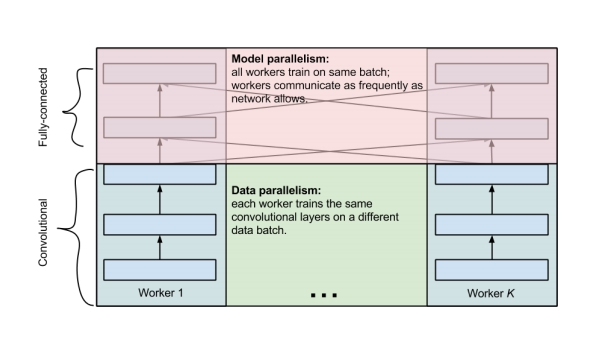
\includegraphics[width=0.4\textwidth]{model_data.png}}
\caption{Model-Parallel and Data-Parallel.\cite{r6}}
\label{fig_model}
\end{figure}

As for parallel optimization based on software implementation, it is widely accepted that model-parallel and data-parallel are the two categories of parallel computing, corresponding to the computing procedure of models \cite{in6}. As shown in Fig.\ref{fig_model}, model-parallel is realized by breaking the models apart, so that minor computing tasks or different parts of the models can be implemented on multiple devices. Data-parallel divides data into groups to be processed separately, and combine the results at the very end. Hybrid systems combining model-parallel and data-parallel technologies are also well developed since there is not a clear-cut distinction between these them. To meet the intention of our course plan, we consider to focus on software improvement by applying pipeline into deep learning frameworks like Deep Neural Networks.

Among commonly used methods to develop parallelism in deep learning frameworks, pipeline takes the advantage of both model-parallel and data-parallel, which will be displayed later in this paper. With proposing a preliminary that many computing process can be regarded as topological graphs, they could be easily serialized by applying a topological sorting algorithm and be converted to an equivalent parallel implementation in pipeline. Besides, since pipeline parallize the program at the instruction level, it can be implemented on hardware, along with the technology of super scalar and multi-issue. Thus, a radical shift from single-core processors to heterogeneous multi-core processors with the technologies listed above is already taking place. 

\section{Related Work}

In order to keep up the booming demand of real-world applications, huge amount of efforts for both model-parallel and data-parallel have been made to improve the parallelization of Deep Learning. For instance, various approaches have been proposed to speed up the training process of ImageNet \cite{r1}, a well-known and applied framework in Deep Learning, especially in Computer Vision. Priya Goyal et.al. \cite{r2} achieved ResNet-50 training in an hour utilizing 256 GPUs. Yang You et. al. \cite{r3} further improved the performance by finishing training in 20 minutes using 2048 Intel Xeon Phi 7250 Processors. Chris Ying et. al. \cite{r4} abridged the training time to 2 minutes after implementing the algorithm on 1024-chip TPUs. The most updated result is 90 seconds, realized by Peng Sun et. al. \cite{r5} with 512 GPUs. Many other works have been conducted to parallelize various deep learning algorithms. 

For Deep Convolutional Neural Network(CNN), all of the work mentioned took reference on the work done by Alex Krizhevsky \cite{r6}. It is one of the earliest but most fundamental work on parallelizing deep CNN. Yet, it started out from the perspective of breaking up CNN structure. In this project, we aim to review and analyze this work thoroughly from the view of pipelining. 

\section{Methods}

We define a sequential list of $L$ layers, each of which specifies its model parameters $w_i$, its stateless forward computation function $f_i$, and an optional cost estimation function $c_i$ that estimates the static computation cost of $i-th$ layer given shapes of all inputs to the layer. Neighboring layers can be combined into a composite layer. For example, the composite layer $p_k$ may be composed of consecutive layers from the $i-th$ layer to the $j-th$ layer. In this case, pk’s model parameters would be the union of $w_i, w_{i+1}, \dots, w_j$ and its forward function would be $F_k = f_j \circ \dots \circ f_{i+1} \circ f_i$. The corresponding backpropagation function $B_k$ is derived from $F_k$ using TensorFlow’s automatic symbolic differentiation mechanism. Its cost estimator is constructed based on $c_i, c_{i+1}, \dots, c_j$ .

After defining the network layers in terms of model parameter $w_i$, cost estimation function $c_i$ and forward computation function $f_i$, the algorithm partitions the network into $K$ composite layers and places $k-th$ composite layer onto $k-th$ accelerator, where $K$ is the number of partitions users specified. Communication primitives are automatically inserted at the partition boundaries to allow data exchanging between neighboring partitions. The partitioning algorithm is heuristic-based. It simply minimizes the variance of each composite layer’s estimated cost. We expect that better partitioning algorithms can potentially improve the performance.

\begin{figure}[htbp]
\centerline{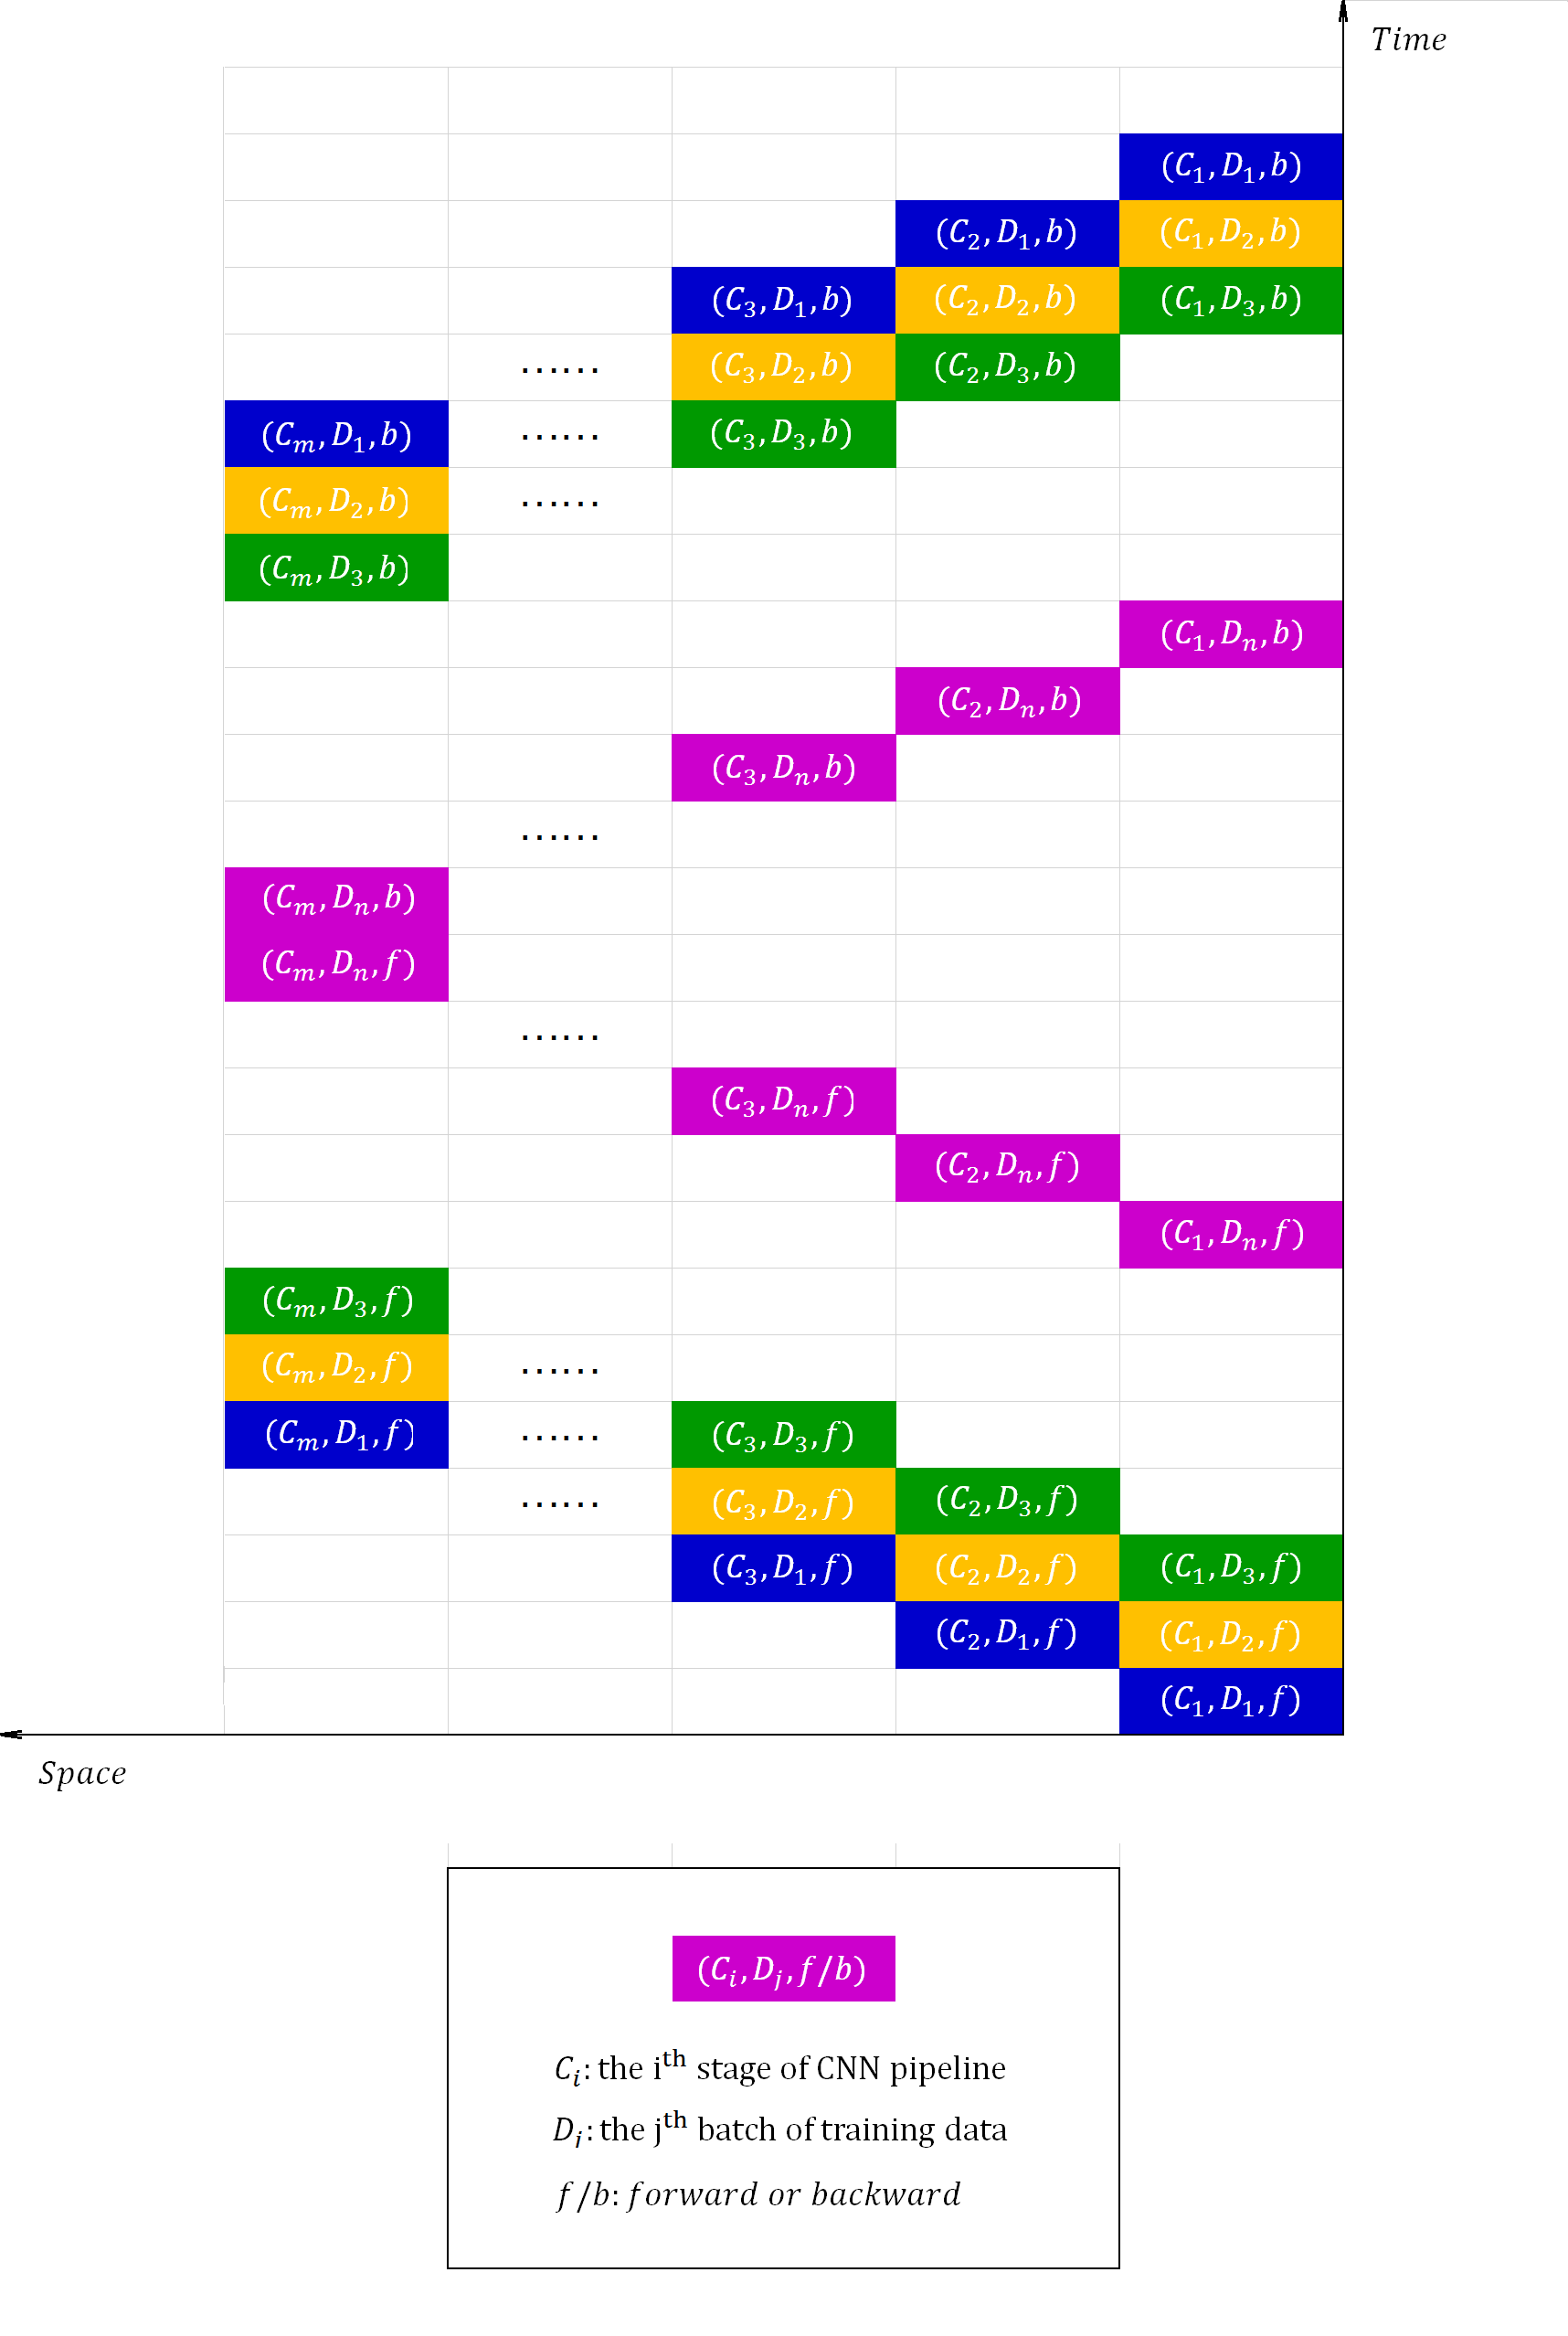
\includegraphics[width = 0.4\textwidth]{pipeline_status.png}}
\caption{Implemented Pipelining Demonstration.}
\label{fig1}
\end{figure}

During training, the algorithm first divides a mini-batch of size $N$ into $T$ micro-batches at the first layer. Each micro-batch contains $N/T$ examples. For instance, an image input tensor with shape $[N, H, W, C]$ is reshaped into $[T, N/T, H, W, C]$. As Fig.\ref{fig1} shows, During the forward pass, the $(k+1)-th$ accelerator starts to compute $F(k+1,t)$ as soon as it finishes the $(t−1)-th$ micro-batch and receives inputs from $F(k,t)$. At the same time, the $k-th$ accelerator can start to compute $F(k,t+1)$.Each accelerator repeats this process $T$ times to finish the forward pass of the whole mini-batch. There are still up to $O(K)$ idle time per accelerator, which we refer to as bubble overhead. This bubble time is $O(K−1, T+K−1)$ and amortized by the number of micro-batches $T$. The last accelerator is also responsible for concatenating the outputs across micro-steps and computing the final loss.

During the backward pass, gradients for each micro-batch are computed based on the same model parameters as the forward pass. Gradients are applied to update model parameters across accelerators only at the end of each mini-batch. Therefore, the algorithm maintains the same synchronous nature of gradient descent, independent of the number of partitions. 

The computation of the backward pass $b_i(x)$ at layer i requires both the upper layer gradients $b_{i+1}(x)$ and cached activations $f_i(x)$. Therefore, the total cached activations need $O(NL)$ space without optimization, where $N$ is the mini-batch size and $L$ is the number of layers in the network. In order to reduce activation memory requirements, the algorithm recomputes the forward passes. Each accelerator only store output activations at the partition boundaries, rather than activations of all intermediate layers within the partition. During the backward pass, the $k-th$ accelerator recomputes the composite forward function $F_k$ and requires only the cache activations at the partition boundaries. As a result, the size of peak activation memory reduces to $O(N +L/K\star N/T)$ where $N/T$ is the micro batch size and $L/K$ is the number of layers in one partition.

The aggregation of the loss during the forward pass introduces a bubble of idleness between the forward and backward passes. The bubble is amortized over the number of micro-steps $T$ In our experiments, we found that the bubble overhead was quite small. This is partly because recomputation during the backward pass can be scheduled earlier without waiting for gradients from earlier layers. However, memory requirements and computation flops at different layers are often quite imbalanced. The activation memory footprint per layer decreases linearly at later layers while the number model parameter per layer increases quadratically. Therefore, imperfect partitioning algorithms will lead to load imbalance when partitioning those layers. Better partitioning algorithms can potentially improve the performance of our heuristic approach.

\section{Results}

We have done the implementation of our idea by TensorFlow and studied the effect of pipelines with $k$ levels, $k \in \{2, 4, 8\}$. Using 42, 000 training images with 28*28 in size, $k$ batches are generated before training. During running, the $k$ layers will dynamically generated and CNN applied 5*5 convolutional cores. The experiment results on a computer with 8 cores and 64GB memory are listed in Table.\ref{tab_result}. As shown, an approximately linear speedup could be achieved when the number of pipeline levels does not exceed the number of cores, yet the consumption of memory is not satisfied, for parameters from different training process are in need of storage in memory simultaneously, which causes redundancy, though parameters of different batches will never commute. Future explorations of DNN parallelism could attempts to improve this situation.

\begin{table}[htbp]
\caption{A Comparative Study of Parallel Implementation}{}
\begin{center}
\begin{tabular}{|c|c|c|c|c|}
\hline
\textbf{Resource}&\multicolumn{4}{|c|}{\textbf{Performance for each Implementation}} \\
\cline{2-5} 
\textbf{Consumption} & \textbf{\textit{Serial}} & \textbf{\textit{2-Pipeline}} & \textbf{\textit{4-Pipeline}} & \textbf{\textit{8-Pipeline}}\\
\hline
Total Time (minutes) & 9.4 & 5.5 & 2.9 & 1.7\\
\hline
Speedup Radio & - & 1.71x & 3.24x & 5.53x\\
\hline
Total Memory (MB) & 632 & 4030 & 7999 & 14623 \\
\hline
Extra Required Memory & - & 6.38x & 12.66x & 23.14x \\
\hline
% \multicolumn{4}{l}{$^{\mathrm{a}}$Sample of a Table footnote.}
\end{tabular}
\label{tab_result}
\end{center}
\end{table}

\begin{figure}[htbp]
\centerline{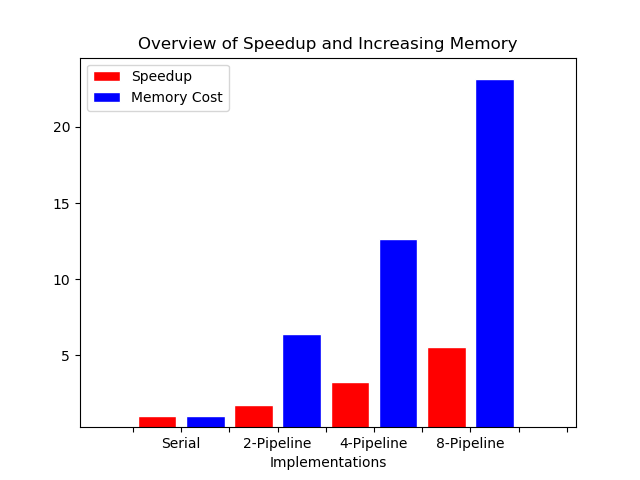
\includegraphics[width=0.4\textwidth]{result.png}}
\caption{An Overview of Speedup and Extra Required Memory.}
\label{fig_hyper}
\end{figure}

\begin{thebibliography}{00}
\bibitem{in1} Marcin Andrychowicz, Bowen Baker, Maciek Chociej, Rafal Jozefowicz, Bob McGrew, Jakub Pachocki, et. al. “Learning Dexterous In-Hand Manipulation”. arXiv preprint arXiv: 1808.00177. 2019.
\bibitem{in2} Lasse Espeholt, Hubert Soyer, Remi Munos, Karen Simonyan, Volodymyr Mnih, Tom Ward, et. al. “IMPALA: Scalable Distributed Deep-RL with Importance Weighted Actor-Learner Architectures”. arXiv preprint arXiv:1802.01561. 2018.
\bibitem{in3} Edie Rasmussen. “Introduction: Parallel processing and information retrieval”. Information Processing and Management . 1991.
\bibitem{in4} Galip Aydin and Ibrahim Riza Hallac, “Distributed NLP”. Third International Symposium on Innovative Technologies in Engineering and Science, Valencia, Spain. 2015.
\bibitem{in5} Maxim Naumov, “Parallel Complexity of Forward and Backward Propagation”. arXiv preprint arXiv:1712.06577.
\bibitem{in6} Peter S.Pacheco (2011) An Introduction to Parallel Programming, Morgan Kaufmann ISBN: 0123742609, 9780123742605
\bibitem{r6} Alex Krizhevsky, “One Weird Trick for Parallelizing Convolutional Neural Networks”. arXiv preprint arXiv: 1404.5997. 2014.
\bibitem{r1} Jia Deng, Wei Dong, Richard Socher, Li-Jia Li, Kai Li and Fei-Fei Li, “ImageNet: A Large-Scale Hierarchical Image Database”. IEEE Computer Vision and Pattern Recognition (CVPR), 2009.
\bibitem{r2} Priya Goyal, Piotr Dollar, Ross Girshick, Pieter Noordhuis, Lukasz Wesolowski, Aapo Kyrola, et. al. “Accurate, Large Minibatch SGD: Training ImageNet in 1 Hour”. arXiv preprint arXiv: 1706.02677. 2017.
\bibitem{r3} Yang You, Zhao Zhang, Cho-Jui Hsieh, James Demmel, Kurt Keutzer. “ImageNet Training in Minutes”, Proceedings of the 47th International Conference on Parallel Processing. 2018.
\bibitem{r4} Chris Ying, Sameer Kumar, Dehao Chen, Tao Wang, Youlong Cheng. “Image Classification at Supercomputer Scale”. NIPS. 2018.
\bibitem{r5} Peng Sun, Wansen Feng, Ruobing Han, Shengen Yan, Yonggang Wen, “Optimizing Network Performance for Distributed DNN Training on GPU Clusters: ImageNet/AlexNet Training in 1.5 Minutes”. arXiv preprint arXiv:1902.06855. 2019.
\end{thebibliography}

\vspace{12pt}

\end{document}
